\section{Vektoren}
\subsection{Definition von Vektoren}
\begin{defi}{Vektoren}{}\index{Vektoren!Definition}
Die Menge aller parallelen, gleich langen und gleich gerichteten Pfeile nennt man Vektor. Jeder Pfeil ist der Repräsentant des Vektors.
\begin{center}

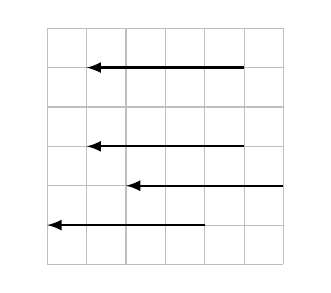
\begin{tikzpicture}[x=.5cm, y=.5cm,domain=-9:9,smooth, cross/.style={draw, cross out,
  minimum size=2*(#1-1pt), inner sep=0pt, outer sep=0pt},>=latex, font= \footnotesize]
   %Raster zeichnen
   \draw [color=gray!50]  [step=5mm] (-1,-1) grid (5,5);

\coordinate(a) at (4,4);
\coordinate(b) at (0,4);

\coordinate(c) at (4,2);
\coordinate(d) at (0,2);

\coordinate(e) at (5,1);
\coordinate(f) at (1,1);

\coordinate(g) at (3,0);
\coordinate(h) at (-1,0);
%Vektor
\draw[thick, ->] (a) node[right]{} -- (b) node[left]{};
\draw[thick, ->] (c) node[right]{} -- (d) node[left]{};
\draw[thick, ->] (e) node[right]{} -- (f) node[left]{};
\draw[thick, ->] (g) node[right]{} -- (h) node[left]{};
\end{tikzpicture}
\end{center}
Alle drei Pfeile sind Repräsentanten des selben Vektors.
\end{defi}
\begin{merke}{Bezeichnungen}{}\index{Vektoren!Bezeichnung}
Vektoren werden mit kleinen lateinischen Buchstaben und einem pfeil gekennzeichnet $\vec{u}$. Verläuft ein Repräsentant eines Vektors von einem Punkt z.B. $P$ zu einem zweiten Punkt z.B. $Q$, so bezeichnet man alle Repräsentanten mit $\vv{PQ}$.
\begin{center}

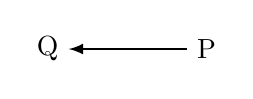
\begin{tikzpicture}[x=.5cm, y=.5cm,domain=-9:9,smooth, cross/.style={draw, cross out,
  minimum size=2*(#1-1pt), inner sep=0pt, outer sep=0pt},>=latex, ]
   %Raster zeichnen
% \draw [color=gray!50]  [step=5mm] (0,0) grid (3,3);
\coordinate(a) at (3,3);
\coordinate(b) at (0,3);
%Vektor
\draw[thick, ->] (a) node[right]{P} -- (b) node[left]{Q};
\end{tikzpicture}
\end{center}
\end{merke}
\begin{satz}{Vektoraddition}{}\phantomsection\label{vekadd}\index{Vektoren!Addition}
Bei der Addition von zwei Vektoren wird an den Endpunkt eines Repräsentanten des ersten Vektors $\vv{a}$ der Beginn eines Repräsentanten des zweiten Vektors $\vv{b}$ gesetzt. Der Pfeil des Summenvektors $\vv{c} = \vv{a} + \vv{b}$ ergibt sich durch den Pfeil der am Anfangspunkt des Vektors $\vv{a}$ beginnt und am Endpunkt des Vektors $\vv{b}$ endet.\\
Da es für einen Vektor unendlich viele Repräsentanten gibt, gibt es immer einen, der an der \glqq richtigen\grqq{} Stelle für eine Addition liegt.
\begin{center}
 
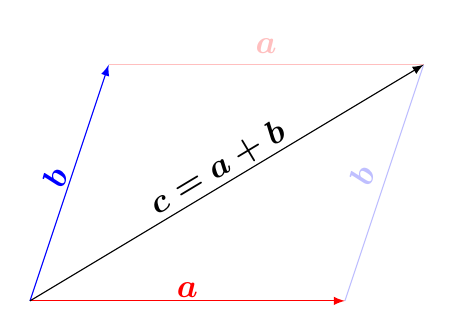
\begin{tikzpicture}[font=\boldmath]\large
    % Punkte
    \coordinate (A) at (0,0) {};
    \coordinate (B) at (4,0) {};
    \coordinate (C) at (1,3) {};
    \coordinate (D) at (5,3) {};

    % Draw the triangle
    \draw[blue!25]  (B) -- (D) node[sloped,midway,above] {$\vv{b}$};
    \draw[red!25]   (C) -- (D) node[sloped,midway,above] {$\vv{a}$};;
    \draw[->,  red,   arrows={-latex}]  (A) -- (B) node[sloped,midway,above=-0.1cm] {$\vv{a}$};
    \draw[->,  blue,  arrows={-latex}]  (A) -- (C) node[sloped,midway,above=-0.1cm] {$\vv{b}$};
    \draw[->, black, arrows={-latex}]  (A) -- (D) node[sloped,midway,above=-0.1cm] {$\vv{c} = \vv{a} + \vv{b} $};
\end{tikzpicture}
\end{center}
\end{satz}
\begin{satz}{Kommutativgesetz der Vektoraddition}{}\phantomsection\label{komuvekadd}
  Wie aus der Zeichnung bei Satz \ref{vekadd} leicht ersichtlich ist, ist die Addition von Vektoren kommutativ. Es gilt also: $$\vv{a} + \vv{b} = \vv{b} +\vv{a}$$ 
\end{satz}
\begin{satz}{Kommutativgesetz der Vektoraddition}{}
  Wie aus der Zeichnung bei Satz \ref{vekadd} leicht ersichtlich ist, ist die Addition von Vektoren kommutativ. Es gilt also: $$\vv{a} + \vv{b} = \vv{b} +\vv{a}$$ 
\end{satz}

\begin{satz}{Assoziativgesetz der Vektoraddition}{}\phantomsection\label{assivekadd}
\begin{center}
 Bei der Addition von Vektoren gilt das Assoziativgesetz. Es gilt also:
 $$(\vv{a} + \vv{b}) + \vv{c} = \vv{a} + (\vv{b} + \vv{c}) = \vv{a} + \vv{b} +\vv{c}$$
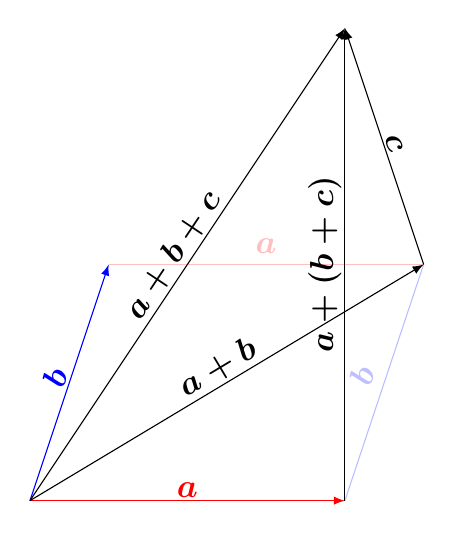
\begin{tikzpicture}[font=\boldmath]\large
    % Punkte
    \coordinate (A) at (0,0) {};
    \coordinate (B) at (4,0) {};
    \coordinate (C) at (1,3) {};
    \coordinate (D) at (5,3) {};
    \coordinate (E) at (4,6) {};

    % Draw the triangle
    \draw[blue!25]  (B) -- (D) node[sloped,midway,above] {$\vv{b}$};
    \draw[red!25]   (C) -- (D) node[sloped,midway,above] {$\vv{a}$};
    \draw[->,  red,   arrows={-latex}]  (A) -- (B) node[sloped,midway,above=-0.1cm] {$\vv{a}$};
    \draw[->,  blue,  arrows={-latex}]  (A) -- (C) node[sloped,midway,above=-0.1cm] {$\vv{b}$};
    \draw[->, black, arrows={-latex}]  (A) -- (D) node[sloped,midway,above=-0.1cm] {$ \vv{a} + \vv{b} $};
    \draw[->,  black,   arrows={-latex}]  (D) -- (E) node[sloped,midway,above=-0.1cm] {$\vv{c}$};
    \draw[->,  black,   arrows={-latex}]  (A) -- (E) node[sloped,midway,above=-0.1cm] {$\vv{a} + \vv{b} + \vv{c}$};
     \draw[->,  black,   arrows={-latex}]  (B) -- (E) node[sloped,midway,above=-0.1cm] {$\vv{a} + (\vv{b} + \vv{c})$};
\end{tikzpicture}
\end{center}
\end{satz}
\begin{b8d}{Besondere Vektoren}{}\index{Vektoren!Nullvektor}\index{Vektoren!Gegenvektor}
Bei der Rechnung mit Vektoren gibt es zwei besondere Vektoren zu betrachten. Hierbei handelt es sich um den sogenannten Nullvektor und den Gegenvektor.\\
Der Nullvektor $\vv{o}$ ist derjenige Vektor, der die Länge Null hat und bei dem sich bei er Addition mit anderen Vektoren nichts ändert. Es gilt: $$\vv{a} +\vv{o} = \vv{o} +\vv{a} = \vv{a}$$
Der Gegenvektor $-\vv{a}$ ist derjenige Vektor, der genauso lang wie der Vektor $\vv{a}$ ist allerdings entgegengerichtet. Für den Gegenvektor $-\vv{a}$ und den Vektor $\vv{a}$ gilt: $$\vv{a} +( -\vv{a} ) =\vv{a}-\vv{a}= \vv{o}$$
\end{b8d}
\begin{bem}{Vektorkette}{}\index{Vektoren!Vektorkette}
Werden mehrere Vektoren addiert so werden die jeweiligen Repräsentanten aneinandergereiht und das Ergebnis nennt man dann Vektorkette.
\end{bem}
\subsection{Vektor und Skalar}
\begin{merke}{Skalar}{}\index{Vektoren!Skalar}
   In der Analytischen Geometrie versteht man unter einem Skalar eine beliebige reelle Zahl. 
\end{merke}
\begin{defi}{Skalare Multiplikation}{}\index{Vektoren!Skalare Multiplikation}
Ein Vektor kann mit einer reellen Zahl durch eine Multiplikation verknüpft werden. Der Vektor $\lambda \cdot \vv{u}$ ist $|\lambda|$-mal so lang wie der Vektor $\vv{u}$. Dabei gilt für dis Zahl $\lambda$ folgendes $\lambda \in \mathds{R}$.\\
Für $\lambda > 0$ hat der Vektor $\lambda \cdot \vv{u}$ die gleiche Richtung wie der Vektor $\vv{u}$.\\
Für $\lambda < 0$ hat der Vektor $\lambda \cdot \vv{u}$ die entgegengesetzte Richtung wie der Vektor  $\vv{u}$.\\
\begin{center}
\begin{tikzpicture}[font=\boldmath]\large
    % Punkte
    \coordinate (A) at (0,0) {};
    \coordinate (B) at (2,1) {};
    \coordinate (C) at (6,2) {};
    \coordinate (D) at (2,0) {};
    \draw[->,  arrows={-latex}]  (A) -- (B) node[sloped,midway,above=-0.1cm] {$\vv{u}$};
    \draw[->,  arrows={-latex}]  (D) -- (C) node[sloped,midway,above=-0.1cm] {$2\cdot \vv{u}$};   
\end{tikzpicture}
\end{center}
\end{defi}
\begin{satz}{Rechenregeln für das Skalarprodukt}{}\index{Vektoren!Skalare Multiplikation}
Die Skalare Multiplikation folgt zwei Gesetzmäßigkeiten. dabei gilt $\lambda, \mu \in \mathds{R}$:
\begin{itemize}
    \item Assoziativgesetz: $\lambda \cdot \left(\mu \cdot \vv{u}\right) =\left( \mu \cdot \lambda \right)\vv{u}$
    \item Distributivgesetz 1: $\lambda \cdot \left(\vv{u} + \vv{v}\right) =\lambda \cdot \vv{u} + \lambda \cdot \vv{v} $
    \item Distributivgesetz 2: $\left( \lambda + \mu\right) \cdot \vv{u} =\lambda \cdot \vv{u} + \mu \cdot \vv{u}  $
\end{itemize}
\end{satz}
\begin{bem}{}{}
Beim aufstellen einer Vektorkette versucht man den Anfangs- und Endpunkt eines Vektors durch bekannte Vektoren zu verbinden. Der Vektor $\vv{AB}$ beginnt im Punkt $A$ und endet im Punkt $B$.

\end{bem}
\begin{bsp}{Vektorkette}{}
Die Vektoren $\vv{a}=\vv{AB}, \vv{b}=\vv{AD}$ und $\vv{c}=\vv{AS}$  spannen eine vierseitige Pyramide ABCDS auf, deren Grundfläche ein Parallelogramm ABCD ist. Der Fußpunkt der Pyramidenhöhe ist der Schnittpunkt der Diagonalen der Grundfläche.   
\begin{center}
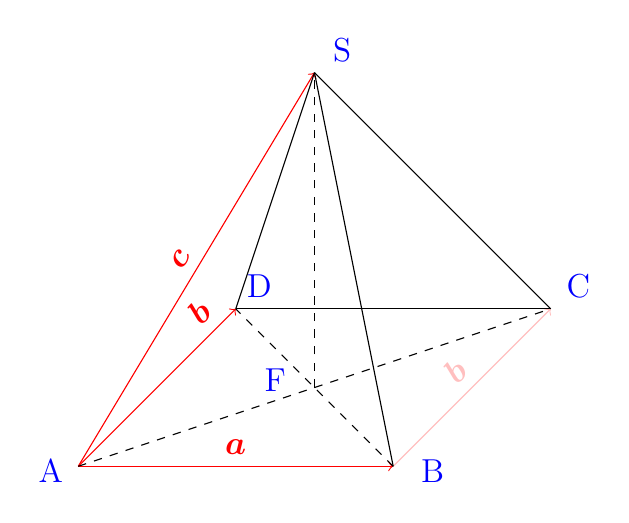
\begin{tikzpicture}[font=\boldmath]\large
    % Punkte
    \coordinate (A) at (0,0) {};
     \draw[blue] (-0.35,-0.35)   node [above] {A};
    \coordinate (B) at (4,0) {};
    \draw[blue] (4.5,-0.35)   node [above] {B};
    \coordinate (C) at (6,2) {};
    \draw[blue] (6.35,2)   node [above] {C};
    \coordinate (D) at (2,2) {};
    \draw[blue] (2.3,2)   node [above] {D};
    \coordinate (E) at (3,5) {};
    \draw[blue] (3.35,5)   node [above] {S};
    \coordinate (F) at (3,1) {};
    \draw[blue] (2.5,0.8)   node [above] {F};
    \draw[->, red]  (A) -- (B) node[sloped,midway,above] {$\vv{a}$};
    \draw[->,red!25]  (B) -- (C) node[sloped,midway,above] {$\vv{b}$};
    \draw  (C) -- (D) node[] {};
    \draw[->,red]  (A) -- (D) node[sloped,above,very near end] {$\vv{b}$};
   \draw[->,red]  (A) -- (E) node[sloped,midway,above] {$\vv{c}$};
   \draw  (E) -- (B) node[] {};
   \draw  (E) -- (C) node[] {};
   \draw  (E) -- (D) node[] {};
   \draw[dashed]  (A) -- (C) node[] {};
   \draw[dashed]  (B) -- (D) node[] {};
   \draw[dashed]  (F) -- (E) node[] {};

\end{tikzpicture}
\end{center}
Folgende Aufgaben sind typisch für Vektorketten
\begin{enumerate}
    \item Warum repräsentieren die Vektoren $\vv{BS}, \vv{CS}$ und $\vv{DS}$ \textcolor{red}{nicht} den Vektor $\vv{c}$?
    \begin{itemize}
        \item $\vv{BS}, \vv{CS}$ und $\vv{DS}$ sind gleich lang wie $\vv{c}$
        \item aber nicht \textcolor{red}{parallel} zu $\vv{c}$
    \end{itemize}
    \item Drücke die Vektoren $\vv{BS}, \vv{CS}, \vv{DS}$ und $\vv{AF}$ mithilfe der Vektoren $\vv{a}, \vv{b}$ und $\vv{
    c}$ aus.
    \begin{itemize}
        \item $\vv{BS}$
        \begin{itemize}
            \item[$\circ$] Um vom Startpunkt $B$ zum Endpunkt $S$ zu kommen, muss man von $B$ nach $A$ und dann nach $S$ \glqq laufen\grqq{}
            \item[$\circ$] $\vv{BS} = -\vv{a} + \vv{c} = \vv{c} - \vv{a}$
        \end{itemize}       
        \item $\vv{CS}$ 
        \begin{itemize}
            \item[$\circ$] Der Vektor $\vv{BC}$ ist ein Repräsentatnt des Vektors $\vv{b}$ 
            \item[$\circ$] $\vv{CS} = -\vv{b} - \vv{a} + \vv{c} = \vv{c} - \vv{a} -\vv{b}$
        \end{itemize}
        \item $\vv{DS}$ 
        \begin{itemize}
            \item[$\circ$] $\vv{DS} = -\vv{b} + \vv{c} = \vv{c} - \vv{b}$
        \end{itemize}
         \item $\vv{AF}$ 
         \begin{itemize}
             \item[$\circ$] Der Punkt $F$ liegt in der Mitte des Vektors $\vv{AC}$
             \item[$\circ$] $\vv{AC} = \vv{a} + \vv{b}$
             \item[$\circ$] $\vv{AF} = \dfrac{1}{2} \left(\vv{a} + \vv{b} \right)$
         \end{itemize}
    \end{itemize}
    \end{enumerate}
 In der Pyramide ist $M$ der Mittelpunkt der Seitenkante $\vv{BS}$ und $N$ der Mittelpunkt der Seitenkante  $\vv{CS}$.  
      \begin{enumerate}
        \item[3.] Drücke den Vektor $\vv{FN}$ mithilfe der Vektoren $\vv{a}, \vv{b}$ und $\vv{
    c}$ aus.
    \end{enumerate}
   \begin{multicols}{2}
    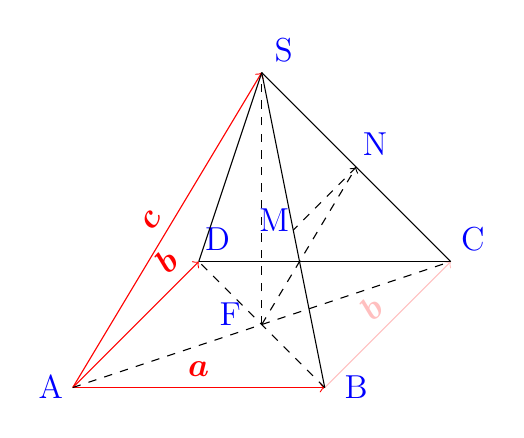
\begin{tikzpicture}[font=\boldmath, scale=0.8]\large
    % Punkte
    \coordinate (A) at (0,0) {};
     \draw[blue] (-0.35,-0.35)   node [above] {A};
    \coordinate (B) at (4,0) {};
    \draw[blue] (4.5,-0.35)   node [above] {B};
    \coordinate (C) at (6,2) {};
    \draw[blue] (6.35,2)   node [above] {C};
    \coordinate (D) at (2,2) {};
    \draw[blue] (2.3,2)   node [above] {D};
    \coordinate (E) at (3,5) {};
    \draw[blue] (3.35,5)   node [above] {S};
    \coordinate (F) at (3,1) {};
    \draw[blue] (2.5,0.8)   node [above] {F};
    \coordinate (G) at (4.5,3.5) {};
    \draw[blue] (4.8,3.5)   node [above] {N};
    \coordinate (H) at (3.5,2.5) {};
    \draw[blue] (3.2,2.3)   node [above] {M};
    \draw[->, red]  (A) -- (B) node[sloped,midway,above] {$\vv{a}$};
    \draw[->,red!25]  (B) -- (C) node[sloped,midway,above] {$\vv{b}$};
    \draw  (C) -- (D) node[] {};
    \draw[->,red]  (A) -- (D) node[sloped,above,very near end] {$\vv{b}$};
   \draw[->,red]  (A) -- (E) node[sloped,midway,above] {$\vv{c}$};
   \draw  (E) -- (B) node[] {};
   \draw  (E) -- (C) node[] {};
   \draw  (E) -- (D) node[] {};
   \draw[dashed]  (A) -- (C) node[] {};
   \draw[dashed]  (B) -- (D) node[] {};
   \draw[dashed]  (F) -- (E) node[] {};
    \draw[dashed]  (G) -- (H) node[] {};
    \draw[->,dashed]  (F) -- (G) node[] {};
\end{tikzpicture} 
    \begin{itemize}
        \item[$\circ$] Vektorkette von $F$ nach $C$ zu $N$.
     \begin{equation*}
            \begin{split}
                \vv{FN} &= \vv{FC} + \vv{CN}\\
                &=\vv{AF} + \dfrac{1}{2} \vv{CS}\\
                &= \dfrac{1}{2} \left(\vv{a} + \vv{b} \right) + \dfrac{1}{2}\left(\vv{c} - \vv{a} -\vv{b}\right)\\
                &=\dfrac{1}{2} \vv{a} + \dfrac{1}{2} \vv{b} + \dfrac{1}{2} \vv{c} - \dfrac{1}{2} \vv{a} -\dfrac{1}{2} \vv{b} \\
                &= \dfrac{1}{2}\vv{c}
            \end{split}
        \end{equation*}
        
    \end{itemize}
   \end{multicols}
   \begin{itemize}
       \item[$\circ$] Daraus folgt, dass der Vektor $\vv{FN}$ parallel und gleichgerichtet zum Vektor $\vv{c}$ aber nur halb so lang ist.
   \end{itemize}
   \begin{enumerate}
    \item[4.] Drücke den Vektor $\vv{MN}$ mithilfe der Vektoren $\vv{a}, \vv{b}$ und $\vv{
    c}$ aus.
    \begin{multicols}{2}
    \begin{itemize}
        \item[$\circ$] Vektorkette von $M$ über $B, C$ zum Punkt $N$.
     \begin{equation*}
            \begin{split}
                \vv{MN} &= - \dfrac{1}{2}\vv{BS} + \vv{BC} + \dfrac{1}{2} \vv{CS}\\
                &= -\dfrac{1}{2} \left( \vv{c} - \vv{a}\right) +\vv{b} + \dfrac{1}{2} \left(\vv{c} - \vv{a} -\vv{b}\right)\\
                &= -\dfrac{1}{2} \vv{c} +\dfrac{1}{2} \vv{a} +\vv{b} + \dfrac{1}{2} \vv{c} - \dfrac{1}{2}\vv{a} -\dfrac{1}{2}\vv{b}\\
                &= \dfrac{1}{2} \vv{b}
            \end{split}
        \end{equation*}  
        \item[$\circ$] Damit folgt, das die Mittellinie $\overline{MN}$ parallel, gleichgerichtet aber nur halb so lang wie der Vektor $\vv{b}$ ist.
    \end{itemize}
    \end{multicols}
\end{enumerate}
\end{bsp}
\section{Der Vektorraum}
\begin{defi}{Der Vektorraum}{}\index{Vektoren!Vektorraum}
    Die Menge aller Vektoren, in der die Gesetze der Addition von Vektoren und deren Multiplikation mit Skalaren gelten, nennt man Vektorraum. Die Basis des Vektorraums setzt sich aus der minimalen Anzahl von Vektoren zusammen die man braucht, um alle anderen Vektoren darstellen zu können. Die Anzahl dieser Vektoren bildet die Dimension des Vektorraums.
\end{defi}
\begin{merke}{Das orthonormale Koordinatensystem}{}\index{Vektoren!orthonormales Koordinatensystem}
    Das zweidimensionale und das dreidimensionale Koordinatensystem der Schulgeometrie ist ein orthonormales Koordinatensystem. Das bedeutet, die Basis besteht aus 2 bzw. 3 Vektoren der Länge eins welche paarweise senkrecht aufeinander stehen. Man bezeichnet diese Vektoren mit $\vv{e}_1, \vv{e}_2, \vv{e}_3$. 
\end{merke}
\begin{b8d}{Die Basisvektoren}{}v\index{Vektoren!Basisvektoren}
Für die Basisvektoren $e_1, e_2$ und $e_3$ gilt folgende Darstellung:\\
$$\vv{e}_1 =\begin{pmatrix} 1 \\ 0 \\0 \end{pmatrix}, 
\vv{e}_2 =\begin{pmatrix} 0 \\ 1 \\0 \end{pmatrix}, 
\vv{e}_3 =\begin{pmatrix} 0 \\ 0 \\1 \end{pmatrix}$$
Mit den Basisvektoren ist man in der Lage, jeden Vektor durch eine Addition der Basisvektoren darzustellen. Diese Darstellung bezeichnet man als Spaltendarstellung der Vektoren. Der Vektor $\vv{a}$ hat damit die Darstellung $\vv{a} = \begin{pmatrix} a_1 \\ a_2 \\a_3 \end{pmatrix} = a_1\cdot \vv{e}_1 + a_2 \cdot \vv{e}_2 + a_3\cdot \vv{e}_3$ mit $a_1, a_2, a_3 \in \mathds{R}$. Die reellen Zahlen $a_i$ nennt man Koordinanten des Vektors $\vv{a}$.  
\end{b8d}
\begin{bem}{Rechnungen mit Vektoren}{}
\begin{itemize}
    \item Addition von Vektoren in der Spaltenschreibweise: Die Vektoren der $\vv{a}$ und $\vv{b}$ werden wie folgt addiert: $$\vv{a} + \vv{b} = \begin{pmatrix} a_1 \\ a_2 \\a_3 \end{pmatrix} + \begin{pmatrix} b_1 \\ b_2 \\b_3 \end{pmatrix} = \begin{pmatrix} a_1 + b_1 \\ a_2 + b_2 \\a_3 + b_3 \end{pmatrix}$$ dabei gilt $a_i, b_i \in \mathds{R}$.
    \item Multiplikation eines Vektors mit einem Skalar: Ein Vektor wird mit einem Skalar wie folgt multipliziert $$\lambda \cdot \vv{a} = \lambda \cdot \begin{pmatrix} a_1 \\ a_2 \\a_3 \end{pmatrix} = \begin{pmatrix} \lambda \cdot a_1 \\ \lambda \cdot a_2 \\\lambda \cdot a_3 \end{pmatrix}$$ mit $\lambda , a_i \in \mathds{R}$.
\end{itemize}
\end{bem}
\begin{satz}{Ortsvektoren}{}\index{Vektoren!Ortsvektor}
Jeder Punkt $P(p_1|p_2|p_3)$ mit $p_i \in \mathds{R}$ des dreidimensionalen Vektorraums lässt sich wie folgt in der Spaltenschreibweise schreiben:
$$\vv{P} = \begin{pmatrix} p_1 \\ p_2 \\p_3 \end{pmatrix}.$$ 
Dieser Vektor repräsentiert genau einen Pfeil der im Urpsrung des Koordinatensystems beginnt und an den Koordinaten des Punktes $P$ endet.\\ 
Diesen Pfeil nennt man Ortsvektor des Punktes $P$.
\end{satz}
\begin{satz}{Verbindungsvektoren}{}
Wird durch den Punkt $A(a_1|a_2|a_3)$ der Anfangspunkt und durch den Punkt $B(b_1|b_2|b_3)$ der Endpunkt eines Vektors festgelegt, so nennt man den dadurch entstehenden Vektor $\vv{AB}$ einen Verbindungsvektor. \\
Die Koordinaten des Verbindungsvektors berechnen sich wie folgt: $$\vv{AB} = \vv{B} -\vv{A} = \begin{pmatrix} b_1 \\ b_2 \\b_3 \end{pmatrix} - \begin{pmatrix} a_1 \\ a_2 \\a_3 \end{pmatrix} = \begin{pmatrix} b_1 - a_1 \\b_2 - a_2 \\b_3 -a_3 \end{pmatrix}$$
für alle $a_i, b_i \in \mathds{R}$.
\end{satz}
\begin{bsp*}{Orts- und Verbindungsvektor}{}

Gegeben sind die Punkte $P,R$ und $S$ im euklidischen Koordinatensystem. Die Punkte haben folgende Koordinaten: $P(2|3|2), R(3|3|0)$ und $S(0|4|2)$. Damit ergeben sich die die Ortsvektoren:
$$\vv{P} = \begin{pmatrix} 2 \\ 3 \\2 \end{pmatrix}, \vv{R} = \begin{pmatrix} 3 \\ 3 \\0 \end{pmatrix}, \vv{S}=\begin{pmatrix} 0 \\4 \\2 \end{pmatrix}.$$ Die Koordinaten des Verbindungsvektors berechnen sich damit wie folgt:
$$\vv{RS} = \vv{S} - \vv{R} = \begin{pmatrix} 0 \\4 \\2 \end{pmatrix} - \begin{pmatrix} 3 \\ 3 \\0 \end{pmatrix}=  \begin{pmatrix} -3 \\ 1 \\2 \end{pmatrix}$$
\tdplotsetmaincoords{70}{120}
\begin{tikzpicture}[scale=2, tdplot_main_coords, axis/.style={-> }, 
vector/.style={-stealth,red}, 
vector guide/.style={dashed,red}]
% -- remove these 3 lines if no axis is preferred
\draw[axis] (0, 0, 0) -- (5, 0, 0) node [left] {$x_1$};
\draw[axis] (0, 0, 0) -- (0, 5, 0) node [above] {$x_2$};
\draw[axis] (0, 0, 0) -- (0, 0, 2) node [above] {$x_3$};
% define points
\coordinate  (d1) at (0,0,0){};
\coordinate  (d2) at (4,0,0){};
\coordinate  (d3) at (2,3,2){};
\coordinate  (d4) at (0,4,2){};
\coordinate  (d5) at (3,3,0){};
\draw[blue] (2,3,2)   node [above] {$P$};
\draw[vector] (d1) -- (d3);
 %\draw (0,0,0) -- ++(-2.5pt,-2.5pt) -- ++(5pt,5pt) ++(-5pt,0pt) -- ++(5pt,-5pt);
  %\draw (2,3,2) -- ++(-2.5pt,-2.5pt) -- ++(5pt,5pt) ++(-5pt,0pt) -- ++(5pt,-5pt);
\draw[vector] (d5) -- (d4);
\draw[blue] (3,3,0)   node [above] {$R$};
\draw[blue] (0,4,2)   node [above] {$S$};
\draw[vector, blue, dashed] (d1) -- (d4);
\draw[vector, blue, dashed] (d1) -- (d5);
\draw[blue] (1.5,1.5,0)   node [above] {$\vv{R}$};
\draw[blue] (0,2,0.6)   node [above] {$\vv{S}$};
\draw[blue] (0,1,0.6)   node [above] {$\vv{P}$};
\end{tikzpicture}
\end{bsp*}
Durch die Verwendung von Koordinaten in der Vektorgeometrie ist es möglich spezielle Punkte relativ einfach zu berechnen. So ist es jetzt möglich, dass man zum Beispiel eine den Mittelpunkt einer Strecke bestimmt oder eine Strecke zu verdoppeln.
\begin{b8d*}{Eigenschaften einer Strecke}{}
Für den Ortsvektor $\vv{M}$ des Mittelpunktes der Strecke $\overline{AB}$ gilt: $$\vv{M} = \dfrac{1}{2}\left(\vv{A} + \vv{B}\right).$$
Die Strecke $\overline{AB}$ lässt sich so, einfach in beliebig viele Teile einteilen. 
\end{b8d*}
\begin{bsp*}{Teilungen einer Strecke}{}
Die Punkte $A$ und $B$ mit den Koordinaten $\vv{A} = \begin{pmatrix} 4 \\0 \\2 \end{pmatrix}$ und $\vv{B}= \begin{pmatrix} -2 \\3 \\5 \end{pmatrix}$ bestimmen eine Strecke $\overline{AB}$. Um die Strecke in vier gleich große Teile einzuteilen bestimmt man als erstes den Mittelpunkt. $$\vv{M_1}=\dfrac{1}{2}\left(\vv{A} + \vv{B}\right) = \dfrac{1}{2}\left( \begin{pmatrix} 4 \\0 \\2 \end{pmatrix} +  \begin{pmatrix} -2 \\3 \\5 \end{pmatrix} \right)= \dfrac{1}{2}\begin{pmatrix} 2 \\3 \\7 \end{pmatrix} = \begin{pmatrix} 1 \\1,5 \\3,5 \end{pmatrix}. $$ 
Anschließend werden die Mittelpunkte der Strecken $\overline{AM_1}$ und $\overline{M_1B}$ berechnet.
$$\vv{M_2} = \dfrac{1}{2}\left(\vv{A} + \vv{M_1}\right) =  \dfrac{1}{2} \left( \begin{pmatrix} 4 \\0 \\2 \end{pmatrix}  + \begin{pmatrix} 1 \\1,5 \\3,5 \end{pmatrix} \right) = \dfrac{1}{2} \begin{pmatrix} 5 \\1,5 \\5,5 \end{pmatrix} = \begin{pmatrix} 2,5 \\0,75 \\2,75 \end{pmatrix}$$
$$\vv{M_3} = \dfrac{1}{2}\left(\vv{M_1} + \vv{B}\right) =  \dfrac{1}{2} \left( \begin{pmatrix} 1 \\1,5 \\3,5 \end{pmatrix} +   \begin{pmatrix} -2 \\3 \\5 \end{pmatrix} \right) = \dfrac{1}{2} \begin{pmatrix} -1 \\4,5 \\8,5 \end{pmatrix} =  \begin{pmatrix} -0,5 \\2,25 \\4,25 \end{pmatrix}$$
Durch die Berechnung der Punkte ergeben sich 4 gleich große Teilstücke. \\
Die Strecken $\overline{AM_2}, \ \overline{M_2M_1}, \ \overline{M_1M_3}$ und $\overline{M_3B}.$
\begin{center}
 
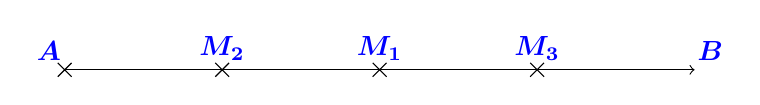
\begin{tikzpicture}[font=\boldmath]
    % Punkte
    \coordinate (C) at (1,3) {};
    \coordinate (D) at (9,3) {};   
    
    \draw[->]  (C) -- (D) node[sloped,midway,above] {};
    \draw[blue] (0.8,3)   node [above] {$A$};
    \draw (1, 3) -- ++(-2.5pt,-2.5pt) -- ++(5pt,5pt) ++(-5pt,0pt) -- ++(5pt,-5pt);
    \draw[blue] (9.2,3)   node [above] {$B$};
       % \draw (9, 3) -- ++(-2.5pt,-2.5pt) -- ++(5pt,5pt) ++(-5pt,0pt) -- ++(5pt,-5pt);
 \draw[blue] (5,3)   node [above] {$M_1$};
        \draw (5, 3) -- ++(-2.5pt,-2.5pt) -- ++(5pt,5pt) ++(-5pt,0pt) -- ++(5pt,-5pt);
 \draw[blue] (3,3)   node [above] {$M_2$};
        \draw (3, 3) -- ++(-2.5pt,-2.5pt) -- ++(5pt,5pt) ++(-5pt,0pt) -- ++(5pt,-5pt);
 \draw[blue] (7,3)   node [above] {$M_3$};
        \draw (7, 3) -- ++(-2.5pt,-2.5pt) -- ++(5pt,5pt) ++(-5pt,0pt) -- ++(5pt,-5pt);     
\end{tikzpicture} 
\end{center}
\end{bsp*}
Die Eigenschaften der Berechnung der Mittelpunkte lassen sich auch auf Flächen und Körper anwenden. So ist es jetzt möglich, den Schwerpunkt eines Dreiecks bzw. den Schwerpunkt einer dreiseitigen Pyramide zu bestimmen.
\begin{merke}{Schwerpunkte bei Strecke, Dreieck und Pyramide}{}\index{Schwerpunkt!Strecke}\index{Schwerpunkt!Dreieck}
\index{Schwerpunkt!Pyramide}
\begin{center}
Mithilfe dieser Übersicht ist es möglich, die Ortskoordinaten des Schwerpunkts zu berechnen.\\[0.5cm]
\bgroup
\def\arraystretch{1.5}%  1 is the default, change whatever you need
\begin{tabular}{|l|c|c|}
    \hline
    & Berechnung & Teilverhältnis \\[0.2cm]
     \hline
     \hline
     Schwerpunkt einer Strecke & $\vv{S_{AB}} = \dfrac{1}{2}(\vv{A} + \vv{B})$ & 1:1\\[0.2cm]
     \hline
     Schwerpunkt eines Dreiecks &$ \vv{S_{ABC}} = \dfrac{1}{3} (\vv{A} + \vv{B} + \vv{C})$ & 1:2\\[0.2cm]
     \hline
     Schwerpunkt einer Pyramide & $\vv{S_{ABCD}} = \dfrac{1}{4}(\vv{A} + \vv{B} +\vv{C} + \vv{D})$ & 1:3\\[0.2cm]
     \hline
\end{tabular}
\egroup
\end{center}
Das Teilverhältnis gibt an, in welchem Verhältnis der Schwerpunkt die einzelnen Teilstrecke unterteilt. So entstehen, zum Beispiel bei der Teilung einer Strecke, zwei gleich lange Teilstrecken.
\end{merke}
\section{Skalar- und Vektorprodukt}
\subsection{Das Skalarprodukt}
Um die Abstände im Raum berechnen zu können wird die Länge eines Vektors definiert.
\begin{defi}{Der Betrag eines Vektors}{}
Gegeben ist der Vektor $\vv{a}$ durch die Koordinaten $\vv{a} = \begin{pmatrix} a_1 \\a_2 \\a_3\end{pmatrix}$. Der Betrag des Vektors entspricht der Länge eines Repräsentanten des Vektors. Hierbei berechnet sich die Länge wie folgt: $$|\vv{a}| = \sqrt{a_1^2 + a_2^2 + a_3^2}$$
\end{defi}
Mit dem Betrag eines Vektors kann jetzt der Abstand zweier Punkte berechnet werden.
\begin{merke}{Abstand zweier Punkte}{}\index{Abstand zweier Punkte}
Durch die Berechnung des Betrags ist es möglich die Entfernung zweier Punkte im Raum zu berechnen. Dadurch haben die Punkte $A(a_1|a_2|a_3)$ und $B(b_1|b_2|b_3)$ die Entfernung: $$|\vv{AB}|=|\vec{B} - \vv{A}| = | \begin{pmatrix} b_1 \\b_2 \\b_3\end{pmatrix} -\begin{pmatrix} a_1 \\a_2 \\a_3\end{pmatrix}| = |\begin{pmatrix} b_1 - a_1 \\b_2 - a_2 \\b_3- a_3\end{pmatrix}| =\sqrt{(b_1-a_1)^2+ (b_2-a_2)^2 + (b_3-a_3)^2}$$
\end{merke}
\begin{bsp}{Berechnung von Längen}{}
Gegeben sind die Punkte $A(2|3|-1)$ und $B(-2|2|1)$. Der Orstvektor des Punktes $A$ hat damit die Länge $$|\vv{A}| = \sqrt{2^2 +3^2 +(-1)^2} = \sqrt{14}\ [LE]$$ und die Punkte $A$ und $B$ haben damit den Abstand $$|\vv{AB}| = |\begin{pmatrix} -2 \\2 \\1\end{pmatrix} - \begin{pmatrix} 2 \\3 \\-1\end{pmatrix}| = |\begin{pmatrix} -4 \\-1 \\2\end{pmatrix}| = \sqrt{(-4)^2 +(-1)^2 + (2)^2} = \sqrt{21} \ [LE]$$
\end{bsp}
Durch die Einführung des Abstands zweier Punkte ist man jetzt in der Lage neues Strukturen im Raum zu definieren. 
\begin{b8d}{Kugelgleichung}{}\index{Kugelgleichung}
Alle Punkte, die von einem gegeben Punkt $M(m_1|m_2|m_3)$ die gleiche Entfernung $r$ haben, liegen auf einer Kugel um den Mittelpunkt $r$. Die Koordinaten aller dieser Punkte $X(x_1|x_2|x_3)$ genügen folgender Gleichung: $$(x_1-m_1)^2 + (x_2 -m_2)^2 + (x_3 -m_3 ^2) = r^2$$
\end{b8d}
In der analytischen Geometrie ist es oft wichtig zu wissen, ob zwei Vektoren senkrecht aufeinander stehen. Diese Information ist mit Hilfe des Skalarprodukts bestimmbar.
\begin{merke}{Das Skalarprodukt}{}\index{Vektoren!Skalarprodukt}
Die Zahl $$\vv{a} \circ \vv{b} = \begin{pmatrix} a_1 \\a_2 \\a_3\end{pmatrix} \circ \begin{pmatrix} b_1 \\b_2 \\b_3\end{pmatrix} = a_1\cdot b_1 + a_2\cdot b_2 + a_3\cdot b_3$$ heißt Skalarprodukt der Vektoren $\vv{a}$ und $\vv{b}$. 
\end{merke}
Damit zwei Vektoren orthogonal bzw. senkrecht zueinander sind, muss für zwei Vektoren $\vv{a}$ und $\vv{b}$ folgende Gleichung gelten: $|\vv{a}|^2 + |\vv{b}|^2 = |\vv{b} -\vv{a}|^2$. Durch eine einfache Umformung der Gleichung folgt\\ $ a_1\cdot b_1 + a_2\cdot b_2 + a_3\cdot b_3 = 0$ und damit ergibt sich folgendes Kriterium.
\begin{b8d}{Orthogonalität von zwei Vektoren}{} \index{Vektoren!Orthogonalität}
Zwei vom Nullvektor verschiedene Vektoren $\vv{a}$ und $\vv{b}$ sind genau dann orthogonal zueinander, wenn ihr Skalarprodukt den Wert Null hat.
\end{b8d}
Schließen zwei Vektoren $\vv{a}$ und $\vv{b}$ einen von $90^{\circ}$ verschiedenen Winkel $\varphi$ ein, so lässt sich dieser wie folgt berechnen.
\begin{merke}{Winkel zwischen zwei Vektoren}{}
Der Winkel $\varphi$ zwischen zwei vom Nullvektor verschiedenen Vektoren $\vv{a}$ und $\vv{b}$ ergibt sich aus folgendem Zusammenhang: $$\cos{\varphi} = \dfrac{\vv{a} \circ \vv{b}}{|\vv{a}| \cdot |\vv{b}|}\hspace{0.5cm}\text{mit}\hspace{0.25cm} 0^{\circ} \leq \varphi \leq 180^{\circ}.$$ 
Die Größe des Winkels $\varphi$ bestimmt sich damit durch die Gleichung:
$$\varphi = \arccos{(\dfrac{\vv{a} \circ \vv{b}}{|\vv{a}| \cdot |\vv{b}|})} = \cos^{-1}{(\dfrac{\vv{a} \circ \vv{b}}{|\vv{a}| \cdot |\vv{b}|})}$$
\end{merke}
\begin{bsp}{Berechnung des Winkels zwischen zwei Vektoren}{}
Gegeben sind die Punkte $A(7|-3|4), B(2|2|4)$ und $C(2|-3|-1)$ die ein Dreieck festlegen. Berechne die Größe des Winkels $\alpha$.
\begin{center}
\begin{tikzpicture}
  \draw
    (3,-1) coordinate (a) node[right] {B}
    -- (0,0) coordinate (b) node[left] {A}
    -- (2,2) coordinate (c) node[above right] {C}
    -- (3,-1) 
    pic[draw=red, ->,  angle radius=1cm]
    {angle=a--b--c};
    \draw
    (0.4,0.2) coordinate (wink) node[right] {$\alpha$};
\end{tikzpicture}
\end{center}
Vorgehen zum berechnen des Winkels $\alpha$:
\begin{enumerate}
    \item Bestimmung der Vektoren $\vv{a} = \vv{AB}$ und $\vv{b} = \vv{AC}$.
    \begin{equation*}
        \begin{split}
            \vv{a} &= \vv{B} - \vv{A} = \begin{pmatrix} 2 \\2 \\4\end{pmatrix} -\begin{pmatrix} 7 \\-3 \\4\end{pmatrix} = \begin{pmatrix} -5 \\5\\0\end{pmatrix} 
            \end{split}
            \end{equation*}
    \begin{equation*}
        \begin{split}
            \vv{b} &= \vv{C} - \vv{A} = \begin{pmatrix} 2 \\-3 \\-1\end{pmatrix} -\begin{pmatrix} 7 \\-3 \\4\end{pmatrix} = \begin{pmatrix} -5 \\0\\-5\end{pmatrix} 
            \end{split}
            \end{equation*}
                
    \item Berechnung des Skalarprodukts.
    \begin{equation*}
        \begin{split}
            \vv{a} \circ \vv{b} &= \begin{pmatrix} -5 \\5 \\0\end{pmatrix} \circ \begin{pmatrix} -5 \\0 \\-5 \end{pmatrix} = 25 +0 +0 = 25
            \end{split}
            \end{equation*}
    \item Berechnung der Beträge der Vektoren $\vv{a}$ und $\vv{b}$.
    \begin{equation*}
        \begin{split}
            |\vv{a}| & = |\begin{pmatrix} -5 \\0\\-5\end{pmatrix}| =  \sqrt{(-5)^2 + (5)^2 + 0^2}  = \sqrt{25+25} = \sqrt{50} = 5\cdot \sqrt{2}\\
            |\vv{b}| &= |\begin{pmatrix} -5 \\0\\-5\end{pmatrix} |= \sqrt{(-5)^2 + 0^2 + (-5)^2} = \sqrt{25+25}= \sqrt{50} = 5\cdot \sqrt{2}
            \end{split}
            \end{equation*}
    \item Bildung des Quotienten und Berechnung des Winkels.
    \begin{equation*}
        \begin{split}
            \cos{(\alpha)} &= \dfrac{\vv{a}\circ \vv{b}}{|\vv{a}| \cdot |\vv{b}|}= \dfrac{25}{5\sqrt{2} \cdot 5\sqrt{2}}\\
            &= \dfrac{25}{50} = \dfrac{1}{2}\\
            \alpha &= \arccos{(\dfrac{1}{2})} = 60^{\circ}
            \end{split}
            \end{equation*}
\end{enumerate}
\end{bsp}
\subsection{Das Vektorprodukt}
\index{Vektoren!Vektorprodukt}
Das Vektorprodukt ist anders als das Skalarprodukt ein Vektor und keine Zahl. Gekennzeichnet wird das Vektorprodukt durch $\times$ statt durch das Multiplikationszeichen $\cdot$. \\
\begin{b8d*}{Vektorprodukt und Skalarprodukt}{}
Dadurch ergibt sich folgende Regel:\\
Bei der Schreibweise $\vv{a} \times\vv{b}$ ergibt sich ein Vektor $\vv{c}$,\\
bei der Schreibweise $\vv{a} \cdot \vv{b}$ ergibt sich eine Zahl $c\in \mathds{R}$.
\end{b8d*}
Das Vektorprodukt $\vv{a} \times \vv{b}$ aus den beiden Vektoren $\vv{a}$ und $\vv{b}$ ist ein Vektor, der die folgenden Eigenschaften besitzt.
\begin{merke}{Eigenschaften des Vektorprodukts}{}
   \begin{enumerate}
       \item $\vv{a} \times \vv{b} = 0$, falls der Vektor $\vv{a}$ bzw. der Vektor $\vv{b}$ der Nullvektor ist.
       \item $\vv{a} \times \vv{b} = 0$, falls der Vektor $\vv{a}$ und der Vektor $\vv{b}$ parallel zueinander sind.
       \item Der Betrag des Vektorprodukts gibt den Flächeninhalt des durch die Vektoren $\vv{a} $ und $\vv{b}$ aufgespannten Parallelogramms wieder. Es gilt damit $$F_P=|\vv{a} \times \vv{b} |.$$
       \item Der Flächeninhalt des durch drei Punkte aufgestellten Dreiecks berechnet sich durch den halben Betrag des Vektorprodukts: $$F_{\text{Dreieck}} = \dfrac{1}{2} |\vv{a} \times \vv{b}|$$
       \item Der resultierende Vektor $\vv{c} $ steht senkrecht sowohl auf dem Vektoren $\vv{a} $ als auch auf dem Vektor $\vv{b}$.
   \end{enumerate} 
\end{merke}
\begin{defi*}{Berechnung des Vektorprodukts}{}
Aus zwei Vektoren $\vv{a}\neq 0$ und $\vv{b} \neq 0$ ergibt sich der Vektor durch das Vektorprodukt wie folgt: $$\vv{a} \times \vv{b} = \begin{pmatrix} a_1 \\a_2\\a_3\end{pmatrix} \times \begin{pmatrix} b_1 \\b_2\\b_3\end{pmatrix} = \begin{pmatrix} a_2\cdot b_3 - a_3\cdot b_2 \\a_3\cdot b_1 - a_1\cdot b_3\\a_1\cdot b_2 - a_2\cdot b_1\end{pmatrix}$$
\end{defi*}
\begin{b8d*}{Berechnung des Vektorprodukts}{}
    Bei der Berechnung des Vektorprodukts ist es möglich die obige Variante benutzen oder eine vereinfachte Variante buntzen. Bei dieser Verkürzten Variante werden unter jeden Vektor jeweils die $x_1$ und $x_2$ Koordinaten des Vektors nochmals notiert und die erste Zeile der Vektoren durchgestrichen. Anschließend werden dann die Koordinaten über kreuz multipliziert und dann entsprechende subtrahiert.
\[
\begin{array}[t]{@{}c@{}}
\vv{c}=\begin{pmatrix} a_1 \\ a_2 \\ a_3 \end{pmatrix} \\ a_1 \\ a_2
\end{array}
\times
\begin{array}[t]{@{}c@{}}
\begin{pmatrix} b_1 \\ b_2 \\ b_3 \end{pmatrix} \\ b_1 \\ b_2
\end{array}
=
\begin{pmatrix}
a_2\cdot b_3-a_3\cdot b_2 \\
a_3\cdot b_1-a_1\cdot b_3 \\
a_1\cdot b_2-a_2\cdot b_1
\end{pmatrix}
\] 
\begin{center}
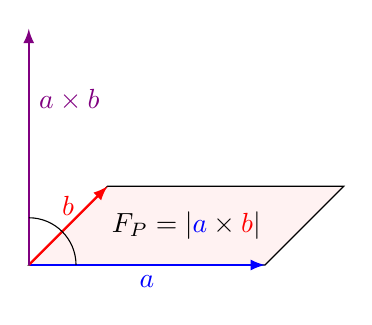
\begin{tikzpicture}
\draw[-,fill=white!95!red](0,0)--(3,0)--(4,1)--(1,1)--cycle;
\node at (2,0.5) {$F_P = |\textcolor{blue}{a}\times \textcolor{red}{b}|$};
\draw[thick,-latex,blue](0,0)--(3,0)node[midway,below]{$a$};
\draw[thick,-latex,red](0,0)--(1,1)node[midway,above]{$b$};
\draw[thick,-latex,blue!50!red](0,0)--(0,3)node[pos=0.7,right]{$a\times b$};
%\draw (0.6,0) arc [start angle=0,end angle=45,radius=0.6]
%node[pos=0.7,right]{$\varphi$};
\draw (0.6,0) arc [start angle=0,end angle=90,radius=0.6]
node[pos=0.7,right]{};
\end{tikzpicture}
\end{center}
\end{b8d*}
\begin{bsp}{Berechnung des Vektorprodukts}{}
Gegeben sind die Punkte $A(3|3|3), B(4|5|6)$ und $C(7|8|9)$. Durch die Bestimmung des Betrags des Vektorprodukts soll der Flächeninhalt des aufgespannten Dreiecks bestimmt werden.
\begin{equation*}
    \begin{split}
        F_{\text{Dreieck}} &= \dfrac{1}{2} \cdot |\vv{AB} \times \vv{AC}|\\
        &= \dfrac{1}{2} \cdot |\begin{pmatrix} 1 \\ 2 \\ 3 \end{pmatrix} \times \begin{pmatrix} 4 \\ 5 \\ 6 \end{pmatrix}|
        = \dfrac{1}{2} \cdot |
\begin{array}[t]{@{}c@{}}
\begin{pmatrix} \bcancel{1} \\ 2 \\ 3 \end{pmatrix} \\ 1 \\ 2
\end{array}
\times
\begin{array}[t]{@{}c@{}}
\begin{pmatrix} \bcancel{4} \\ 5\\ 6 \end{pmatrix} \\ 4 \\ 5
\end{array}|\\
&=
\dfrac{1}{2} \cdot |\begin{pmatrix}
2\cdot 6-3\cdot 5 \\
3\cdot 4-1\cdot 6 \\
1\cdot 5-2\cdot 4
\end{pmatrix}|
=\dfrac{1}{2} \cdot | \begin{pmatrix}
12-15 \\
12-6 \\
5-8
\end{pmatrix}| =\dfrac{1}{2} \cdot |\begin{pmatrix}
-3 \\
6 \\
-3
\end{pmatrix}|\\
&= \dfrac{1}{2} \cdot \sqrt{9+36+9} = \dfrac{1}{2} \cdot \sqrt{54} =\dfrac{3}{2} \cdot \sqrt{6} \ \text{[FE]} 
    \end{split}
\end{equation*}
\end{bsp}
\subsection{Das Spatprodukt}
\index{Vektoren!Spatprodukt}
Ein Spat ist ein geometrischer Körper, der sechs Parallelogramme als Seitenflächen besitzt. Die gegenüberliegende Parallelogramme sind immer kongruent zueinander und liegen in parallelen Ebenen.\\
Unter dem Spatprodukt versteht man das Skalarprodukt eines Vektors mit dem Vektorprodukt zweier weiterer Vektoren.
\begin{defi}{Das Spatprodukt}{}
Spannen die Vektoren $\vv{a}, \vv{b}$ und $\vv{c}$ einen Spat bzw. eine dreiseitige Pyramide auf, ist das Volumen:
$$V_{\text{Spat}} = |(\vv{a}\times\vv{b})\circ \vv{c}|$$ $$V_{\text{Pyramide}}=\dfrac{1}{6}|(\vv{a}\times\vv{b})\circ \vv{c}| $$
\end{defi} 
\begin{bsp}{Berechnung des Volumens einer dreiseitigen Pyramide I}{}
Durch die Vektoren $\vv{a} = \begin{pmatrix} 1\\2\\3
\end{pmatrix}, \vv{b}= \begin{pmatrix}
    2\\3\\1
\end{pmatrix}$ und $\vv{c}= \begin{pmatrix}
   3\\1\\2
\end{pmatrix}$ spannen eine dreiseitige Pyramide auf. Das Volumen dieser Pyramide bestimmt sich damit durch das Spatprodukt wie folgt:
\begin{equation*}
    \begin{split}
      V_{\text{Pyramide}} &= \dfrac{1}{6} \cdot |(\vv{a}\times \vv{b})\circ \vv{c}| = \dfrac{1}{6} \cdot |(\begin{pmatrix}1\\2\\3\end{pmatrix} \times 
\begin{pmatrix} 2\\3\\1 \end{pmatrix}) \circ 
\begin{pmatrix} 3\\1\\2 \end{pmatrix}|\\
&=\dfrac{1}{6} \cdot |\begin{pmatrix} -7\\5\\-1 \end{pmatrix}\circ \begin{pmatrix} 3\\1\\2 \end{pmatrix}|  =\dfrac{1}{6} \cdot |-18| = 3\ \text{[VE]}
    \end{split}
\end{equation*}
\end{bsp}
\begin{b8d*}{Berechnung der Determinante}{}
    Das Spatprodukt lässt sich alternativ durch die Berechnung der sogenannten Determinante bestimmen. Die Determinante bestimmt sich durch folgendes Schema:
\[
\det(\vv{a}, \vv{b}, \vv{c})
%
=\begin{matrix}\begin{tikzpicture}
\matrix [
matrix of math nodes,
column sep=1em,
row sep=1em,
] (sarrus) {
a_1 & b_1 & c_1  \\ a_2 & b_2 & c_2 \\ a_3 & b_3 & c_3 \\
};
% Striche
\path ($(sarrus-1-1.north west)-(0.5em,0)$) edge[] ($(sarrus-3-3.south east -| sarrus-1-1.north west)-(0.5em,0)$);
\path ($(sarrus-1-3.north east)+(0.5em,0)$) edge[] ($(sarrus-3-3.south east -| sarrus-1-3.north east)+(0.5em,0)$);
\end{tikzpicture}\end{matrix}
%
=\begin{matrix}\begin{tikzpicture}
\matrix [
matrix of math nodes,
column sep=1em,
row sep=1em,
%left delimiter={|} %,right delimiter={|}, 
] (sarrus) {
a_1 & b_1 & c_1 & a_1 & b_1 \\ a_2 & b_2 & c_2 & a_2 & b_2\\ a_3 & b_3 & c_3 & a_3 & b_3\\
};
% Striche
\path ($(sarrus-1-1.north west)-(0.5em,0)$) edge[] ($(sarrus-3-3.south east -| sarrus-1-1.north west)-(0.5em,0)$);
\path ($(sarrus-1-3.north east)+(0.5em,0)$) edge[] ($(sarrus-3-3.south east -| sarrus-1-3.north east)+(0.5em,0)$);
\path[->,blue] (sarrus-1-1) edge (sarrus-2-2)
(sarrus-2-2) edge (sarrus-3-3)
(sarrus-1-2) edge (sarrus-2-3)
(sarrus-2-3) edge (sarrus-3-4)
(sarrus-1-3) edge (sarrus-2-4)
(sarrus-2-4) edge (sarrus-3-5);
\path[->,red](sarrus-3-1) edge[dashed] (sarrus-2-2)
(sarrus-2-2) edge[dashed] (sarrus-1-3)
(sarrus-3-2) edge[dashed] (sarrus-2-3)
(sarrus-2-3) edge[dashed] (sarrus-1-4)
(sarrus-3-3) edge[dashed] (sarrus-2-4)
(sarrus-2-4) edge[dashed] (sarrus-1-5);

\foreach \c in{3,4,5} \node[blue] at (sarrus-3-\c.south east) {$+$};
\foreach \c in{3,4,5} \node[red] at (sarrus-1-\c.north east) {$-$};

% Strich rechts
\path ($(sarrus-1-5.north east)+(0.5em,0)$) edge[densely dotted] ($(sarrus-3-5.south east -| sarrus-1-5.north east)+(0.5em,0)$);
\end{tikzpicture}\end{matrix} 
\]
Aus der Determinante folgt damit für das Volumen folgende Rechnung:
\begin{equation*}
    \begin{split}
        V_{\text{Spat}} &= |\det(\vv{a}, \vv{b}, \vv{c})| \\
        &= |a_1\cdot b_2 \cdot c_3 + b_1\cdot c_2 \cdot a_3 + c_1\cdot a_2 \cdot b_3 - a_3\cdot b_2 \cdot c_1 - b_3\cdot c_2 \cdot a_1 - c_3\cdot a_2\cdot b_1|\\
        V_{\text{Pyramide}} &= \dfrac{1}{6}\cdot |\det(\vv{a}, \vv{b}, \vv{c})| \\ 
        &= \dfrac{1}{6}\cdot |a_1\cdot b_2 \cdot c_3 + b_1\cdot c_2 \cdot a_3 + c_1\cdot a_2 \cdot b_3 - a_3\cdot b_2 \cdot c_1 - b_3\cdot c_2 \cdot a_1 - c_3\cdot a_2\cdot b_1|
    \end{split}
\end{equation*}
\end{b8d*}
\begin{bsp}{Berechnung des Volumens einer dreiseitigen Pyramide II}{}
 Durch die Vektoren $\vv{a} = \begin{pmatrix} 1\\2\\3
\end{pmatrix}, \vv{b}= \begin{pmatrix}
    2\\3\\1
\end{pmatrix}$ und $\vv{c}= \begin{pmatrix}
   3\\1\\2
\end{pmatrix}$ spannen eine dreiseitige Pyramide auf. 
\[
\det(\vv{a}, \vv{b}, \vv{c})
%
=\begin{matrix}\begin{tikzpicture}
\matrix [
matrix of math nodes,
column sep=1em,
row sep=1em,
] (sarrus) {
1 & 2 & 3  \\ 2 &3 & 1 \\ 3 & 1 & 2 \\
};
% Striche
\path ($(sarrus-1-1.north west)-(0.5em,0)$) edge[] ($(sarrus-3-3.south east -| sarrus-1-1.north west)-(0.5em,0)$);
\path ($(sarrus-1-3.north east)+(0.5em,0)$) edge[] ($(sarrus-3-3.south east -| sarrus-1-3.north east)+(0.5em,0)$);
\end{tikzpicture}\end{matrix}
%
=\begin{matrix}\begin{tikzpicture}
\matrix [
matrix of math nodes,
column sep=1em,
row sep=1em,
%left delimiter={|} %,right delimiter={|}, 
] (sarrus) {
1 & 2 & 3 & 1 & 2 \\ 2 & 3 & 1 & 2 & 3\\ 3 & 1 & 2 & 3 & 1\\
};
% Striche
\path ($(sarrus-1-1.north west)-(0.5em,0)$) edge[] ($(sarrus-3-3.south east -| sarrus-1-1.north west)-(0.5em,0)$);
\path ($(sarrus-1-3.north east)+(0.5em,0)$) edge[] ($(sarrus-3-3.south east -| sarrus-1-3.north east)+(0.5em,0)$);
\path[->,blue] (sarrus-1-1) edge (sarrus-2-2)
(sarrus-2-2) edge (sarrus-3-3)
(sarrus-1-2) edge (sarrus-2-3)
(sarrus-2-3) edge (sarrus-3-4)
(sarrus-1-3) edge (sarrus-2-4)
(sarrus-2-4) edge (sarrus-3-5);
\path[->,red](sarrus-3-1) edge[dashed] (sarrus-2-2)
(sarrus-2-2) edge[dashed] (sarrus-1-3)
(sarrus-3-2) edge[dashed] (sarrus-2-3)
(sarrus-2-3) edge[dashed] (sarrus-1-4)
(sarrus-3-3) edge[dashed] (sarrus-2-4)
(sarrus-2-4) edge[dashed] (sarrus-1-5);

\foreach \c in{3,4,5} \node[blue] at (sarrus-3-\c.south east) {$+$};
\foreach \c in{3,4,5} \node[red] at (sarrus-1-\c.north east) {$-$};

% Strich rechts
\path ($(sarrus-1-5.north east)+(0.5em,0)$) edge[densely dotted] ($(sarrus-3-5.south east -| sarrus-1-5.north east)+(0.5em,0)$);
\end{tikzpicture}\end{matrix} 
\]
Aus der Determinante folgt damit für das Volumen folgende Rechnung:
\begin{equation*}
    \begin{split}
        V_{\text{Pyramide}} &= \dfrac{1}{6}\cdot |\det(\vv{a}, \vv{b}, \vv{c})| \\ 
        &= \dfrac{1}{6}\cdot |1\cdot 3 \cdot 2 + 2\cdot 1 \cdot 3 + 3\cdot 2 \cdot 1 - 3\cdot 3 \cdot 3 - 1\cdot 1 \cdot 1 - 2\cdot 2\cdot 2|\\
        &= \dfrac{1}{6} \cdot |6+6+6-27-1-8|\\
        &= \dfrac{1}{6} \cdot |-18| = 3 \ \text{[VE]}
    \end{split}
\end{equation*}
\end{bsp}